\section{Discrete Event Simulation}\label{sec:appendix_des}

For the purposes of this study, a discrete event simulation (DES) model was
constructed to support the Markov chain version described in 
section~\ref{sec:queueing_model}.
The queueing model was built in python using the Ciw 
library~\cite{ciwpython}.

The constructed model simulates a queueing system with two waiting spaces and 
two types of individuals. 
The expected behaviour of the nodes in Ciw have been modified such that 
individuals moving from waiting zone 2 into waiting zone 1 get blocked 
if there are more than \(T\) individuals in waiting zone 1.

The same performance measures described in sections 
\ref{sec:waiting_time}, \ref{sec:blocking_time} and 
\ref{sec:proportion_within_target} can also be calculated using the DES model.
The simulation can be ran a number of times to eliminate stochasticity and the
outcomes of the two methods can be directly comparable. 

\subsection{Tutorial: building the DES model}

The DES model is constructed in a generic way that so that it can be used for
any queueing system with two waiting spaces and two types of individuals.
For instance, consider a queueing system with the following parameters, as 
described in section~\ref{sec:queueing_model}:

\begin{multicols}{4}
    \begin{itemize}
        \item \( \lambda_1 = 2 \)
        \item \( \lambda_2 = 3 \)
        \columnbreak
        \item \( \mu = 1 \)
        \item \( C = 6 \)
        \columnbreak
        \item \( T = 10 \)
        \item \( N = 20 \)
        \columnbreak
        \item \( M = 10 \)
    \end{itemize}
\end{multicols}


\begin{figure}[H]
    \centering
    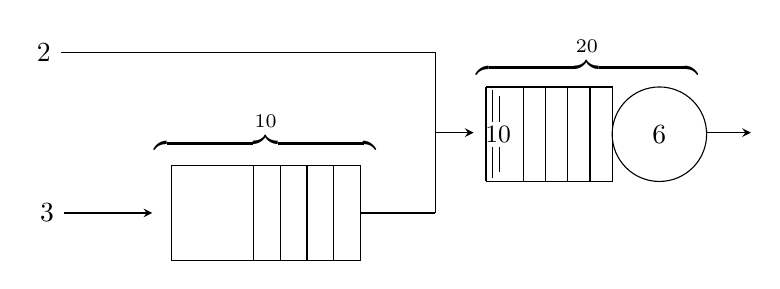
\begin{tikzpicture}[>=stealth, scale=0.8],
        % the rectangle of parking queue
        \draw (0,0) -- ++(3cm,0) -- ++(0,-1.5cm) -- ++(-3cm,0);
        % the vertical lines of parking queue
        \foreach \i in {1,...,4, 7.1}
            \draw (3cm-\i*12pt,0) -- +(0,-1.5cm);
        
        % The label above Queue 1 -> M
        \node[anchor=north] at (1.5cm, 1cm) {\( 
            \overbrace{\qquad \qquad \qquad \qquad}^{10} 
        \)};
        
        % the rectangle in Queue 2
        \draw (5,1.25) -- ++(2cm,0) -- ++(0,-1.5cm) -- ++(-2cm,0);
        % the vertical lines in Queue 2
        \foreach \i in {1,...,4, 5.7}
            \draw (7cm-\i*10pt,1.25) -- +(0,-1.5cm);
        % The two vertical lines at the start of Queue 2 
        \draw (7cm-54pt,1.2) -- +(0,-0.5cm);
        \draw (7cm-54pt,0.3) -- +(0,-0.5cm);        
        \draw (7cm-51pt,1.1) -- +(0,-0.4cm);
        \draw (7cm-51pt,0.3) -- +(0,-0.4cm);

        % The label between the lines for T
        \node[anchor=north] at (5.19, 0.78 cm) {\small{\( 10 \)}};

        % The label above Queue 2 -> N
        \node[anchor=north] at (6.6cm, 2.2cm) {\(
            \overbrace{\qquad \qquad \qquad \qquad}^{20}
        \)};

        % the circle in Queue 2
        \draw (7.75,0.5) circle [radius=0.75cm] node {\(6\)};

        % Arrow line from Queue 2 outside
        \draw[->] (8.5,0.525) -- +(20pt,0);
        
        % Line from lambda_2 to Queue 1
        \draw[<-] (-0.3,-0.75) -- +(-40pt,0) node[left] {\( 3 \)};

        % Lines after Parking queue
        \draw[-] (3,-0.75) -- +(34pt,0);
        \draw (4.2, 0.525) -- (4.2, -0.75);
        
        % Lines for lambda_1 arrivals
        \draw (4.2, 1.8) -- +(-169.5pt,0) node[left] {\( 2 \)};
        \draw (4.2, 1.8) -- (4.2, 0.525);

        % Line from both individuals to Queue 2
        \draw[->] (4.2, 0.525) -- (4.8, 0.525);  
    \end{tikzpicture}
    \caption{A diagrammatic representation of the queueing model example}
    \label{fig:diagram_of_queueing_system_appendix_example}
\end{figure}

This model will be studied by using  
\lstinline[style=pystyle]{ambulance_game}.
Install the created library in your python environment, by running the 
following command in the command line:
\begin{lstlisting}[style=terminalstyle]
    $ pip install ambulance_game
\end{lstlisting}

Having installed the package, the following code can be used to simulate the 
queueing system defined earlier and get all the data records for a single run.

\begin{lstlisting}[style=pystyle]
    
    >>> import ambulance_game as abg
    >>> Simulation = abg.simulation.simulate_model(
    ...     lambda_1=3,
    ...     lambda_2=2,
    ...     mu=1,
    ...     num_of_servers=6,
    ...     threshold=10,
    ...     system_capacity=20,
    ...     buffer_capacity=10,
    ... )
    >>> all_records = Simulation.get_all_records()
    >>> all_records[3]
    Record(id_number=1, customer_class=0, node=2, arrival_date=0.4728763843239206, waiting_time=0.0, service_start_date=0.4728763843239206, service_time=0.5457131455415929, service_end_date=1.0185895298655134, time_blocked=0.0, exit_date=1.0185895298655134, destination=-1, queue_size_at_arrival=0, queue_size_at_departure=4)
\end{lstlisting}

The above block code outputs the fourth individual record from the simulation
object.
The simulation object can be used to view the every event that occurred in the 
simulation 
The data records can then be used to get overall performance measures about the
constructed queueing model.
The overall waiting time that individuals wait in waiting zone 1 can be acquired 
by running:


\begin{lstlisting}[style=pystyle]
    >>> import numpy as np
    >>> mean_wait = np.mean(
    ...    [record.waiting_time for record in all_records if record.node == 2]
    ... )
    0.2246928220731305
\end{lstlisting}

This value is the average waiting time of all the customers in the system for a
single run. 
By nature, discrete event simulation can output different results for different
runs of the same set of parameters.
This stochasticity can be reduced by running the simulation multiple times 
and then getting the mean waiting time from all the runs.

\begin{lstlisting}[style=pystyle]
    >>> all_simulations = abg.simulation.get_multiple_runs_results(
    ...     lambda_1=3,
    ...     lambda_2=2,
    ...     mu=1,
    ...     num_of_servers=6,
    ...     threshold=10,
    ...     system_capacity=20,
    ...     buffer_capacity=10,
    ...     seed_num=0,
    ...     num_of_trials=10,
    ... )
    >>> mean_wait = np.mean(
    ...     [np.mean(w.waiting_times) for w in all_simulations]
    ... )
    0.35037759808989827
\end{lstlisting}


\subsection{How-to guide}

The package can be installed by either running:

\begin{lstlisting}[style=terminalstyle]
    $ pip install ambulance_game
\end{lstlisting}

in the command line or via the instructions provided in the GitHub repository.
% TODO: Cite repository
The required arguments that need to be passed to the simulate\_model() function
are the following:
\begin{itemize}
    \item lambda\_1 (\(\lambda_1\)): The arrival rate of class 1 individuals.
    \item lambda\_2 (\(\lambda_2\)): The arrival rate of class 2 individuals.
    \item mu (\(\mu\)): The service rate of the servers.
    \item num\_of\_servers (\(C\)): The number of servers in the system.
    \item threshold (\(T\)): The threshold that indicates when to start blocking 
    class 2 individuals.
\end{itemize}

To get the simulation object with all the data records, the following code can be
used:
\begin{lstlisting}[style=pystyle]
    >>> import ambulance_game as abg
    >>> Simulation = abg.simulation.simulate_model(
    ...     lambda_1=3,
    ...     lambda_2=2,
    ...     mu=1,
    ...     num_of_servers=6,
    ...     threshold=10,
    ... )
    >>> Simulation.get_all_records()[1]
    Record(id_number=1, customer_class=0, node=2, arrival_date=0.5391449803891563, waiting_time=0.0, service_start_date=0.5391449803891563, service_time=0.17003700443114755, service_end_date=0.7091819848203038, time_blocked=0.0, exit_date=0.7091819848203038, destination=-1, queue_size_at_arrival=0, queue_size_at_departure=0)
\end{lstlisting}

Additional arguments that can be passed to the function are:
\begin{itemize}
    \item \textit{system\_capacity}: The maximum number of individuals in 
    waiting zone 2.
    \item \textit{buffer\_capacity}: The maximum number of individuals in 
    waiting zone 1.
    \item \textit{seed\_num}: The seed number for the random number generator.
    \item \textit{runtime}: How long to run the simulation for.
\end{itemize}

From a single run of the simulation the data records can be used the get the
average for certain performance measures. 
The following code can be used to get the mean waiting time, blocking time, 
service time and the proportion of individuals within target.

\begin{lstlisting}[style=pystyle]
    >>> records = Simulation.get_all_records()
    >>> mean_wait = np.mean(
    ...     [w.waiting_time for w in records]
    ... )
    >>> mean_block = np.mean(
    ...     [b.time_blocked for b in records]
    ... )
    >>> mean_service = np.mean(
    ...     [s.service_time for s in records]
    ... )
    >>> target = 1
    >>> proportion_within_target = np.mean(
    ...     [w.waiting_time <= target for w in records]
    ... )
    
\end{lstlisting}


To eliminate any stochasticity in the simulation, the simulation can be run
numerous times and get the average performance measures out of all the runs.


\begin{lstlisting}[style=pystyle]
    >>> import numpy as np
    >>> import ambulance_game as abg
    >>> all_simulations = abg.simulation.get_multiple_runs_results(
    ...     lambda_1=3,
    ...     lambda_2=2,
    ...     mu=1,
    ...     num_of_servers=6,
    ...     threshold=10,
    ...     system_capacity=20,
    ...     buffer_capacity=10,
    ...     seed_num=0,
    ...     runtime=2000,
    ...     num_of_trials=10,
    ... )
    >>> mean_wait = np.mean([
    ...     np.mean(w.waiting_times) for w in mean_simulations
    ... ])
    >>> mean_service = np.mean([
    ...     np.mean(s.service_times) for s in mult_results
    ... ])
    >>> mean_block = np.mean([
    ...     np.mean(b.blocking_times) for b in mult_results
    ... ])
\end{lstlisting}

To get the average proportion of individuals within target, run the following
code:

\begin{lstlisting}[style=pystyle]
    >>> import ambulance_game as abg
    >>> (
    ...     overall_proportion,
    ...     class_1_proportion,
    ...     class_2_proportion,
    ... ) = abg.simulation.
    get_mean_proportion_of_individuals_within_target_for_multiple_runs(    
    ...     lambda_1=3,
    ...     lambda_2=2,
    ...     mu=1,
    ...     num_of_servers=6,
    ...     threshold=10,
    ...     system_capacity=20,
    ...     buffer_capacity=10,
    ...     seed_num=0,
    ...     num_of_trials=10,
    ...     runtime=2000,
    ...     target=1,
    ... )
\end{lstlisting}
% TODO: Fix code for proportion of individuals within time target

\subsection{Reference}




\subsection{Explanation}

For every service completion Ciw stores all data records in a simulation 
object~\cite{ciwpython}.
For the specific library the records that are stored, along with the 
range of values that they can take are as follows:

\begin{multicols}{2}
    \begin{itemize}
        \item \textbf{id\_number} \(\in R\).
        \item \textbf{customer\_class} \(= 0\)
        \item \textbf{node} \(= \{0, 1, 2, -1 \} \)
        \item \textbf{arrival\_date} \( \in R^+ \)
        \item \textbf{waiting\_time} \( \in R^+ \)
        \item \textbf{service\_start\_date} \( \in R^+ \)
        \item \textbf{service\_time} \( \in R^+ \)
        \item \textbf{service\_end\_time} \( \in R^+ \)
        \item \textbf{time\_blocked} \( \in R^+ \)
        \item \textbf{exit\_date} \( \in R^+ \)
        \item \textbf{destination} \( = \{1, 2, -1\} \)
        \item \textbf{queue\_size\_at\_arrival} \( \in N \)
        \item \textbf{queue\_size\_at\_departure} \( \in N \)
    \end{itemize}
\end{multicols}


% TODO: Archive simulation python code
